\documentclass[12pt]{article}
\usepackage[a4paper, margin=1in]{geometry}
\usepackage[T1]{fontenc}
\usepackage{graphicx}
\usepackage{titlesec}
\usepackage{caption}
\usepackage{subcaption}
\usepackage[section]{placeins}
\usepackage{chngcntr}
\usepackage{sectsty}
\usepackage{algorithmicx}
\usepackage[ruled,vlined]{algorithm2e}
\usepackage[hidelinks]{hyperref}
\usepackage{listings}
\usepackage{xcolor}
\usepackage{amsmath}

\sectionfont{\centering}
\counterwithin{figure}{section}
\renewcommand{\abstractname}{\large Abstract}
\renewcommand{\baselinestretch}{1.5}

\lstset{
    basicstyle=\ttfamily,
    columns=fullflexible,
    breaklines=true,
    postbreak=\mbox{\textcolor{red}{$\hookrightarrow$}\space}
}

\newcommand{\sectionfontstyle}{\fontsize{16pt}{1em}\usefont{T1}{phv}{b}{n}}

\begin{document}
    \pagenumbering{gobble}
    \thispagestyle{empty}
    \begin{center}
        \textit{Project Report on}\\
        \vspace{2mm}
        \Large{\textsc{Sql2Neo: Interconversion of SQL, NoSQL and Neo4j formats}}\\
        \vspace{3mm}
        \textit{Submitted by}\\
        \large{\textbf{
            Aayush Jain (16IT101)\\
            Aditi Rao (16IT103)
        }}\\
        \vspace{4mm}
        Under the Guidance of\\
        \textbf{Shruti J R}\\
        Department of Information Technology, NITK Surathkal\\
        \vspace{4mm}
        \textit{Date of Submission: 11 June 2020}\\
        \vspace{4mm}
        in partial fulfillment for the award of the degree\\
        of\\
        \textbf{Bachelor of Technology}\\
        In\\
        \textbf{Information Technology}\\
        At
        \vspace{4mm}\\
        
\includegraphics[width=1.2in,height=1.2in]{img/nitk.jpg}\\
        \textbf{Department of Information Technology}\\
        \textbf{National Insitute of Technology Karnataka, Surathkal}\\
        June 2020
    \end{center}

    \newpage

    \begin{abstract}
        In order to leverage data relationships and gain insights into the ``big picture'' presented by the data, organizations need a database technology that stores relationship information as a first-class entity. This can be done through the use of Graph Databases such as Neo4j. However, many legacy databases are currently stored in SQL or (more recently) non-graphical NoSQL-based systems, thus removing the possibility of enhanced insights brought about through the use of a graph. Thus, this work details the methodology and implementation of Sql2Neo, a command-line tool to convert data between SQL/NoSQL systems to Neo4j. The resulting database effectively stores data relationships but is also flexible when expanding a data model or conforming to changing business needs. It is uniquely suited to visualization for higher-level decision making and inference mining. Sql2Neo also supports query translation to Neo4j’s Cypher Query Language (CQL) from standard formats such as SQL, increasing the ease of mobility from SQL/NoSQL systems to Neo4j without the rewriting of existing queries. 
    \end{abstract}

    \newpage

    \tableofcontents

    \newpage

    \pagenumbering{arabic}

    \section{\sectionfontstyle Introduction}
    A graph database is an online database management system with Create, Read, Update, and Delete (CRUD) operations working on a graph data model. A graph data model is defined by a collection of nodes representing entities and relationships that connect the nodes. Graph databases are preferred when we want to focus exclusively on understanding the relationship between entities in our database and want to be able to infer data connections without using things like foreign keys or out-of-band processing, such as MapReduce. 

    In order to leverage data relationships and gain insights into the ``big picture'' presented by the data, organizations need a database technology that stores relationship information as a first-class entity. The rigid schemas of legacy relational database management systems (RDBMS) make it difficult to add different connections or adapt to new business requirements. Not only do graph databases effectively store data relationships; they are also flexible when expanding a data model or conforming to changing business needs, and are uniquely suited to visualization for higher-level decision making and inference mining.

    Relational Databases or SQL databases are a  type of DBMS that defines database relationships in the form of tables, also known as relations. They are the most popular DBMS type in the market. Unlike network DBMS, RDBMS does not support many to many relationships. Relational DBMS usually have pre-defined data types that they can support. SQL stands for Structured Query Language and is the standard language for dealing with Relational Databases. It can be used to insert, search, update, and delete database records and many other operations, including optimizing and maintaining databases. Databases like MySQL Database, Oracle, MS SQL Server, Sybase, etc. use SQL.

    NoSQL is an upcoming category of Database Management Systems. It is main characteristic is it is non-adherence to Relational Database Concepts. The popularity of NoSQL databases grew with internet giants such as Google, Facebook, Amazon, etc. who use them to deal with gigantic volumes of data. NoSQL systems are preferred in these cases due to their ability to manage large datasets without performance trade-offs. The alternative to upgrading hardware to fix the problem would be to distribute our database load on multiple hosts as the load increases. This is known as ``scaling out''. NoSQL databases are non-relational databases that scale-out better than relational databases and are designed with web applications in mind. They do not use SQL to query the data and do not follow strict schemas like relational models. Some examples of NoSQL databases include MongoDB, CouchDB, and HBase.
    Neo4j is a graph database management system described as an ACID-compliant transactional database with native graph storage and processing. Neo4j is the most popular graph database used today. Neo4j is implemented in Java and accessible from software written in other languages using CQL through a transactional HTTP endpoint, or through the binary ``bolt'' protocol.

    \newpage

    \section{\sectionfontstyle Literature Survey}
    \subsection{Related Work}
    Singh et al.~\cite{base_paper} propose a methodology to convert a relational to a graph database by exploiting the schema and the constraints of the source, applied in this case to healthcare data. Here, MySQL was used as the source database with the intended target being Neo4j. They reported the notable efficiency of the system designed for querying. They also note that visualization has also significantly improved with the usage of graph databases.

    De Virgilio et al.~\cite{rdbms2graph} also propose a methodology to convert a relational database to a graph database by exploiting the schema and the constraints of the source. The approach also supports the translation of conjunctive SQL queries over the source into graph traversal operations over the target. The methodology describes an automatic conversion system from SQL databases to a graph database which allows the created database to perform better than RDB in certain instances of highly complicated schemas.

    Maity et al.~\cite{nosql2rdbms} view the standard problem of converting the RDBMS to NoSQL in the opposite approach and conceptualize a problem where NoSQL is converted back to an RDBMS based system.  The approach is illustrated using a case study on MongoDB and Neo4j. They note significant successes in conversion using their algorithm and note the potential for its use in not only  NoSQL systems to RDBMS but also for interconversion between two NoSQL systems.

    Vicknair et al.~\cite{db_comparison} report on a comparison of Neo4j with MySQL, for use as the underlying technology in the development of a software system to record and query data provenance information. They noted an almost tenfold increase in speed while using Neo4j for traversal based queries. They conclude that, in general, the graph database did better at the structural type queries and full-text character searches than the relational database. With more development of Neo4j to include integer-based indexing measures as well, it could outperform RDBMS systems in a query on numeric data.

    Batra and Tyagi~\cite{rgdb_compare} also report on the comparative performance of Neo4j and MySQL, noting that the retrieval times of graph databases is less than relational databases as graph databases look only at records that are directly connected to other records. They conclude noting the flexibility of graph databases when new relationships are added as schema restructuring is not required.

    \subsection{Outcome of Literature Survey}
    From the survey, it is clear that the use of graph databases for applications involving a significant focus on entity relationships or visualization would be highly beneficial. It is also evident that it may be useful to transform data from traditional RDBMS to NoSQL systems, such as graph databases solely for the flexibility it offers in terms of the addition of relationships/query speeds for traversal queries. Our proposed methodology aims to allow for quick and easy transformation of existing databases to graph format to take advantage of these benefits. 

    \subsection{Problem Statement}
    Graph database systems such as Neo4j offer various advantages over traditional RDBMS in terms of traversal queries, visualization, and flexibility in defining new relations without schema restructuring. However, a vast majority of applications could benefit from this store data in traditional SQL setups (while some do in newer NoSQL systems). Thus, there is a need to develop a tool to allow for efficient transformation between these systems to graph databases to enhance decision making and insights into the data.

    \subsection{Objectives}
    In order to meet the demands of this problem, our proposed system must meet the following objectives. The system architecture must be designed to allow for \textit{extensibility} in terms of the addition of new SQL/NoSQL systems to convert from. To allow for this, it is necessary to develop a \textit{standard intermediate format} from which conversion to Neo4j can take place. The system must be able to accurately and appropriately \textit{represent relationships} expressed by the use of concepts such as foreign keys in RDBMS, as well as the many to many relationships described in NoSQL systems. The transformation must be done quickly, \textit{without loss of information}, and into a form suitable for direct visualization. There must also be an efficient method for \textit{query translation from SQL/NoSQL based query languages to CQL}, as well as the creation of required indices on identified fields to allow for faster query processing and result retrieval.

    \newpage

    \section{\sectionfontstyle Requirement Analysis}
    Sql2Neo is intended to be a command-line tool that enables interconversion between SQL, NoSQL, and Neo4j formats.

    \subsection{Functional Requirements}
    \begin{enumerate}
        \item [F1.] SQL databases must be fully converted to a Neo4j database. This includes indexes, constraints, records, and relationships.
        \item [F2.] NoSQL databases must be fully converted to a Neo4j database. This includes constraints (inferred) and records.
        \item [F3.] SQL queries must be translated to a Neo4j query to provide interoperability between databases.
    \end{enumerate}

    \subsection{Non-Functional Requirements}
    \begin{enumerate}
        \item [NF1.] Convert NoSQL database to intermediate SQL format to provide compatibility.
        \item [NF2.] Manage data loading from databases in order to prevent memory overuse and overflow errors.
        \item [NF3.] Provide Sql2Neo as an isolated tool (with packaged dependencies) to improve usability.
    \end{enumerate}

    Most software and hardware requirements intersect with the implementation tools, as discussed in section~\ref{sec:impl}.

    \newpage

    \section{\sectionfontstyle System Design/Architecture}
    \label{sec:sys_arch}
    \begin{figure}[htb!]
        \centering
        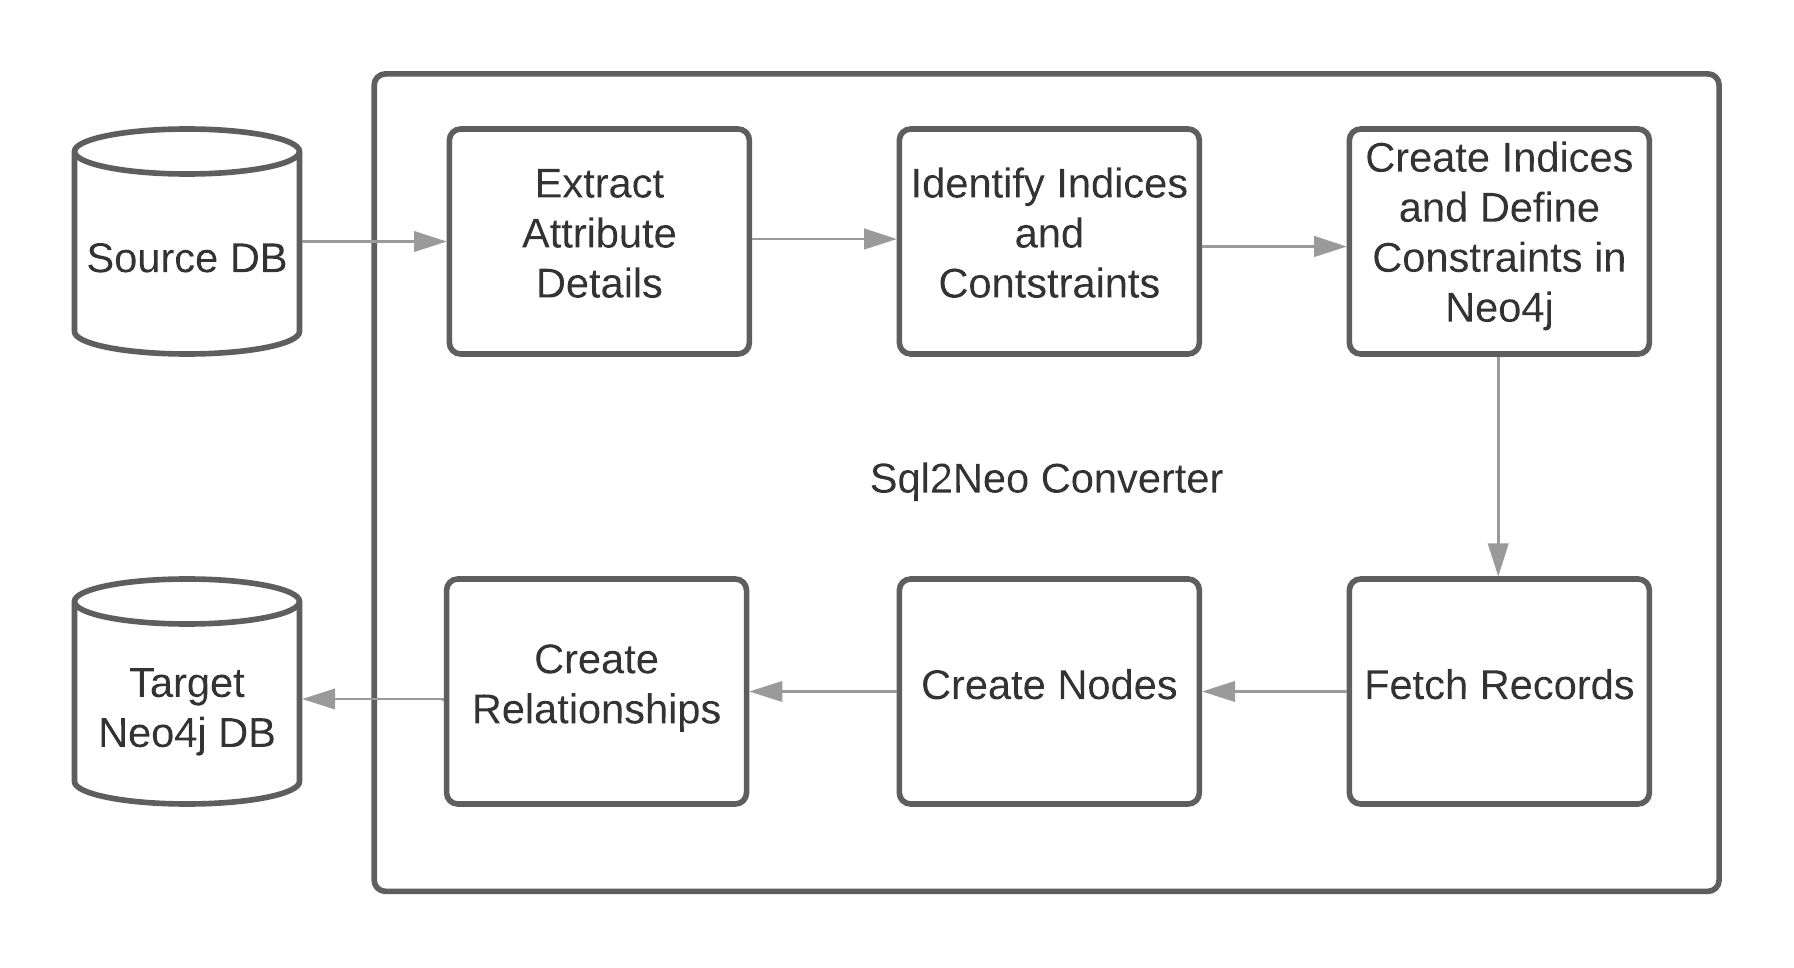
\includegraphics[width=155mm]{img/sql2neo_converter.png}
        \caption{SQL2Neo Data Converter}
        \label{fig:sql2neo_converter}
    \end{figure}

    Figure~\ref{fig:sql2neo_converter} presents an overview of the proposed system architecture. The aim is to take our source database and start by extracting attribute details. This includes information on attribute name, data type (in case conversion is required as Neo4j does not support some data types), uniqueness, a primary/foreign key, or an index that needs to be built on it. Through this, we can further identify indices and constraints in the data, and subsequently, define them as required. At the end of this step, all data description information has been translated to a format which can be further used while translating records into Neo4j.

    Then we begin the population of the Neo4j database. We fetch the records from the source database and, using the data descriptions we have extracted in the previous steps, store it in an intermediate, universal format. This is the last step before node and relationship creation in Neo4j begins.
    
    As Neo4j creates relationships between existing nodes, the nodes are defined first from the identified entities in the data description. Then, relationships or links between the nodes are created and committed to the database.
    
    The system architecture has been designed to encourage extensibility to include compatibility with multiple SQL and NoSQL implementations. All the primary steps before node creation begin to deal with bringing the data to an established universal format, after which conversion to Neo4j entities and relationships is a single pipeline process for all. Thus, it requires that only translation steps to this intermediate format must be determined to include another implementation in the converter.
    
    \begin{figure}[htb!]
        \centering
        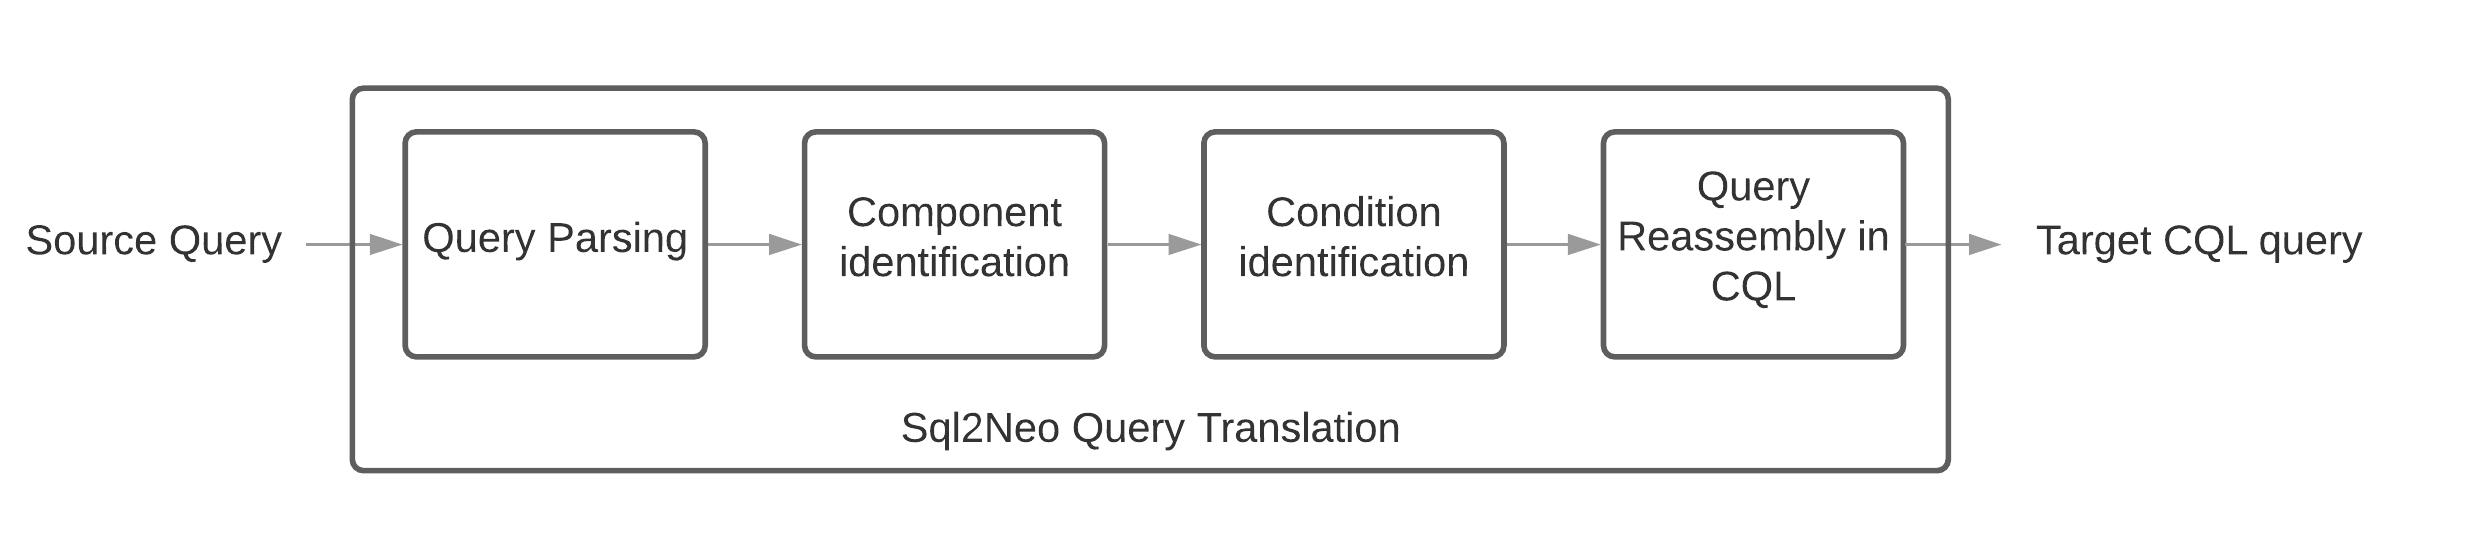
\includegraphics[width=155mm]{img/sql2neo_query.png}
        \caption{SQL2Neo Query Translator}
        \label{fig:sql2neo_query}
    \end{figure}

    In addition, we also undertake query translation from source (SQL/NoSQL) to CQL or Cypher Query Language. The steps begin with parsing the query to isolate terms of interest (figure~\ref{fig:sql2neo_query}). This is followed by identifying components (such as entities and attributes) from the parsed data. We then identify any conditional clauses to be placed (such as found in an SQL ``WHERE'' query phrase) and represent them appropriately. Finally, the query is reassembled from its components and placed into a template structure for an equivalent CQL query.

    \newpage

    \section{\sectionfontstyle Methodology}
    \subsection{Converting SQL-databases to Neo4j format}
    The first step to convert an SQL database is to extract attribute details of each table. This data is available in the \verb|information_schema| of the database. The data for each attribute answers the following questions:
    \begin{itemize}
        \item should this attribute be \textit{indexed}?
        \item does this attribute have a \textit{uniqueness constraint}?
        \item is this attribute a \textit{foreign key reference} to another table's attribute?
    \end{itemize}

    \begin{algorithm}[htb!]
        \SetAlgoLined
        \caption{Extract attribute details of SQL database}
        \KwIn{\textbf{R}, a relational database}
        \KwOut{\textbf{AS}, an attribute set containing details of each attribute}
        AS \gets\ \phi\tcc*{empty map}
        \ForEach{table in \textbf{information\_schema(R)}}{
            AS[table] \gets\ \phi\tcc*{empty map}
            \ForEach{attr in \textbf{table}}{
                AS[table][attr] \gets\ \{index, unique, fk\}\;
            }
        }
        return AS\;
        \label{algo:sql_attr_set}
    \end{algorithm}

    The index and uniqueness constraint data enable the Neo4j set up to be as closely modeled to the relational one. Furthermore, indexing on attributes is maintained across systems, and rigid constraints are also satisfied while inserting in the Neo4j database.

    Since Neo4j stores data as JSON documents, it does not define a rigid and formal schema. Owing to this property, indices, and constraints can be created before the data is actually inserted. In Neo4j, index creation is not idempotent, meaning that creating the index twice results in an error. Additionally, constraints implicitly create an index on the specified attribute (much like relational databases). Thus constraints are applied only on those attributes that are not indexed.

    \begin{algorithm}[htb!]
        \SetAlgoLined
        \caption{Create indices and constraints in Neo4j}
        \KwIn{\textbf{AS}, an attribute set containing details of each attribute}
        \KwResult{\textbf{G}, a graph database with applied indices and constraints}
        \ForEach{table in \textbf{AS}}{
            \ForEach{attr in \textbf{table}}{
                \uIf{attr must be indexed}{
                    CreateIndex(G, table, attr)\;
                }
                \uElseIf{attr has constraint but not indexed}{
                    \tcc*[h]{if attr is indexed, then it meets uniqueness constraint}

                    CreateUniquenessConstraint(G, table, attr)\;
                }
            }
        }
        \label{algo:sql_create_index}
    \end{algorithm}

    \FloatBarrier

    In terms of CQL, \verb|CreateIndex(G, table, attr)| is equivalent to 
    \begin{lstlisting}
        CREATE INDEX index_name ON:table(attr);
    \end{lstlisting}
    \verb|CreateUniquenessConstraint(G, table, attr)| is equivalent to 
    \begin{lstlisting}
        CREATE CONSTRAINT constraint_name ON (t:table) ASSERT t.attr IS UNIQUE;
    \end{lstlisting}

    Conversion of a table's records to Neo4j nodes is a fairly straightforward task. A naive approach is followed where each table's records are converted to a node. This implies that individual tables that behave purely as relationships are also converted to nodes instead of being retained into Neo4j.

    \begin{algorithm}[htb!]
        \SetAlgoLined
        \caption{Populate the graph database with records}
        \KwIn{\textbf{R}, a relational database}
        \KwResult{\textbf{G}, a populated graph database}
        \ForEach{table in \textbf{R}}{
            \ForEach{record in \textbf{table}}{
                CreateNewNode(G, table, record)\;
            }
        }
        \label{algo:sql2graph}
    \end{algorithm}

    \verb|CreateNewNode(G, table, record)| is equivalent to 
    \begin{lstlisting}
        CREATE (t:table $record);
    \end{lstlisting}
    provided that \verb|record| is a map of key-value pairs (record assumed as a parameter).

    Finally, relationship conversion is performed. This step takes the foreign key relations from each table and maps them to a relation in Neo4j. This also means that the semantics of the relation is lost since the edge (in Neo4j) does not provide actual data. Instead, it must be inferred from the database.

    \begin{algorithm}[htb!]
        \SetAlgoLined
        \caption{Create relationships between nodes in the graph data}
        \KwIn{\textbf{AS}, an attribute set containing details of each attribute}
        \KwResult{\textbf{G}, a graph database with relationships}
        \ForEach{table in \textbf{AS}}{
            \ForEach{attr in \textbf{table}}{
                \If{attr is foreign key}{
                    fk\_table, fk\_attr \gets\ GetFKReference(attr)\;
                    CreateRelationship(G, table, attr, fk\_table, fk\_attr)\;
                }
            }
        }
        \label{algo:sql2rel}
    \end{algorithm}

    \verb|CreateRelationship(G, table, attr, fk_table, fk_attr)| is equivalent to 
    \begin{lstlisting}
        MATCH (a:table), (b:fk_table) WHERE a.attr = b.fk_attr CREATE (a) -[r:relationship_name]-> (b);
    \end{lstlisting}

    \subsection{Converting NoSQL-databases to Neo4j format}
    The primary difference between a NoSQL and relational database is that NoSQL databases do not define a formal schema. If data from such a database were to be migrated, it would have lacked constraints and indices. Thus, an additional step is performed as compared to the procedure for RDBMS migration.

    First, the NoSQL database is converted to an intermediate SQL-like format. This intermediate format improves maintainability and allows for seamless management of attribute characteristics over a traditional method.

    \begin{algorithm}[htb!]
        \SetAlgoLined
        \caption{Convert a NoSQL database to a relational format}
        \KwIn{\textbf{N}, a NoSQL database}
        \KwOut{\textbf{AS}, a relational interpretation of \textbf{N}'s attributes}
        AS \gets\ \phi\tcc*{empty map}
        \ForEach{collection, \textbf{C}, in \textbf{N}}{
            AS[C] \gets\ \phi\tcc*{empty map}
            \ForEach{field in \textbf{C}}{
                \If{field has unique values}{
                    AS[C][field] \gets\ \{unique\gets true\}\;
                }
                \If{field not present in each record}{
                    make field nullable
                }
            }
            \uIf{unique field exists}{
                AS[C][field] \gets\ \{index\gets true\}
            }
            \uElseIf{\textbf{C} has unique id}{
                \tcc*[h]{uniqueness is absent}

                use auto-generated id as index\;
            }
            \uElse{
                insert unique id and use as index\;
            }
        }
        return AS\;
        \label{algo:nosql_conversion}
    \end{algorithm}

    A NoSQL can define records in the same collection with a field missing. To convert to a relational model, all such fields are assumed to be nullable, and the missing records are filled in with \verb|NULL| values. Furthermore, the first unique field is taken as the primary key. Many NoSQL databases auto-generate a unique object identifier, which can prove to be useful if a unique field does not exist. Once \verb|AS| is derived from the database, the migration can proceed as per the algorithms defined for SQL databases.

    \subsection{Translating SQL queries to Cypher queries}
    \label{sec:meth_query}
    SQL and Cypher have quite a few common keywords that aid in simpler translation between queries. At its core, query translation requires:
    \begin{enumerate}
        \item identification of queried tables
        \item identification of projection attributes
        \item identification of selection conditions
        \item extracting other keywords that can be translated
    \end{enumerate}

    As mentioned above, few of the keywords shared between SQL and Cypher are \verb|WHERE|, \verb|LIMIT|, \verb|ORDER BY|, \verb|AS|, and \verb|DISTINCT|. In algorithm \ref{algo:query_translate}, tokens are considered to be of two types, namely, \textit{keywords} and \textit{identifiers}. Identifiers follow a keyword normally, and are treated as a list of identifiers. This allows for multiple identifiers to be picked up for translation at once.

    \begin{lstlisting}
        SELECT p.name FROM person p;
        SELECT name FROM person;
    \end{lstlisting}
    The above queries are equivalent, however, Cypher requires node labels to be explicitly provided. So, \verb|MapToVariableName| maps a given list to appropriate variable names (using `n' as default variable).
    \begin{lstlisting}
        MATCH (p:person) RETURN p.name;
        MATCH (n:person) RETURN n.name;
    \end{lstlisting}
    A similar approach is applied to mapping variable names to the \verb|ORDER BY| attributes.

    The algorithm can be extended to include other keywords that exist within CQL, and also to convert other keywords (like JOIN) into Cypher equivalents. The given approach is provided only on \verb|SELECT| queries since commonly used ones may benefit from such a translation.


    \begin{algorithm}[htb!]
        \SetAlgoLined
        \caption{Translate SQL query to CQL}
        \KwIn{\textbf{Q}, an SQL query}
        \KwOut{\textbf{C}, converted Cypher query}
        tokens \gets\ Tokenize(Q)\tcc*{split SQL query into individual tokens (keywords and identifiers)}
        selection \gets\ \verb|NULL|\;
        limit \gets\ \verb|NULL|\;
        order \gets\ \verb|NULL|\;
        \For{token in \textbf{tokens}}{
            \uIf{token is \textbf{SELECT}}{
                attributes \gets\ TokenAfter(token)\;
                attributes \gets\ MapToVariableName(attributes)\tcc*{if table name is not provided (table.attr), then attributes must be mapped to default}
            }
            \uIf{token is \textbf{FROM}}{
                tables \gets\ TokenAfter(token)\;
                tables \gets\ MapToVariableName(tables)\tcc*{if variable name not given to table, provide defaults}
            }
            \uElseIf{token is \textbf{WHERE}}{
                selection \gets\ TokenAfter(token)\;
            }
            \uElseIf{token is \textbf{LIMIT}}{
                limit \gets\ TokenAfter(token)\;
            }
            \uElseIf{token is \textbf{ORDER BY}}{
                order \gets\ TokenAfter(token)\;
                order \gets\ MapToVariableName(order)\tcc*{if table name is not provided (table.attr), then attributes must be mapped to default}
            }
        }
        C \gets\ BuildCypherQuery(tables, attributes, selection, order, limit)\;
        return C\;
        \label{algo:query_translate}
    \end{algorithm}

    \clearpage

    \section{\sectionfontstyle Implementation}
    \label{sec:impl}
    The proposed approach was implemented on a system running Ubuntu 20.04 LTS. The following additional software is used:
    \begin{itemize}
        \item Python 3.8.2
        \begin{itemize}
            \item mysql-connector-python 8.0.20
            \item py2neo 4.3.0
            \item pymongo 3.10.1
            \item python-dotenv 0.13.0
            \item pandas 1.0.4
            \item sqlparse 0.3.1
        \end{itemize}
        \item MySQL v8.0.20 for testing SQL databases
        \item MongoDB v3.6.8 for testing NoSQL databases
        \item Neo4j 4.0.5
    \end{itemize}

    The user decides which database he/she wants to migrate. Details of each database (host, username, password, database name) must be present in a \verb|.env| file. Using the configuration provided here, a connection is established with the source and the target database (Neo4j). As per algorithm~\ref{algo:sql_attr_set}, an attribute set, AS, is maintained that holds data in the following format.
    \begin{lstlisting}
        `trained': {
            `certificationdate': {
                `position': 3, 
                `index': False, 
                `unique': False, 
                `foreign_key': None
            },
            `certificationexpires': {
                `position': 4, 
                `index': False, 
                `unique': False, 
                `foreign_key': None
            },
            `physician': {
                `position': 1, 
                `index': False, 
                `unique': False, 
                `foreign_key': `physician.employeeid'
            },
            `treatment': {
                `position': 2, 
                `index': False, 
                `unique': False, 
                `foreign_key': `procedure_record.code'
            }
        },...
    \end{lstlisting}

    From the above data, it is easy to create indices and constraints on any given attribute.

    Test migration for a MySQL database is carried out on a sample hospital database containing 45 records across 10 tables. This dataset has 13 different foreign key relationships.

    Similarly, for NoSQL, the data is derived in the same format as for MySQL. However, there is an additional cost associated with determining the attribute statistics, i.e., the collected data has to be fully loaded into memory to check for uniqueness. In order to handle loading large datasets in memory, \textit{pandas DataFrames} is used. They can efficiently load large datasets and provide useful methods such as \verb|is_unique| to help determine attribute statistics.

    Testing for MongoDB is done on two databases. The first is a database containing US zip code information with 29353 records. Each record has the same attributes and behaves similar to a relational database. Loading this zip code information into a DataFrame takes negligible time, with the main bottleneck being the creation of 29353 nodes. For the second case, a sample database is created with a badly-defined schema. Multiple attributes are missing in the records of the collection. All these values are created and marked as \verb|None| (\verb|NULL| in Python).

    As mentioned in section \ref{sec:meth_query}, the input queries are first tokenized and then converted to CQL equivalents. Tokenization is performed by the \textit{sqlparse} library. The program allows users to run the queries on the migrated database, or perform a \textit{dry run}, i.e., the user may validate the translated queries. As per the algorithm, the following keywords/features exist:
    \begin{itemize}
        \item Allows for projection attribute aliasing, i.e., p.name AS 'Patient', is retained
        \item Table renaming, i.e., SELECT p.name, nurse.name FROM patient p, nurse n, retains table names defined in SQL
        \item `*' projection is retained and replaced with `RETURN n'
        \item Projection attributes are fully translated
        \item Order by, and limit keywords are retained
    \end{itemize}

    \newpage

    \section{\sectionfontstyle Results and Analysis}
    We perform the conversion on a test MySQL database ``hospital'' as described in the implementation section. The following images display the results upon conversion to a Neo4j graph database.

    \begin{figure}[htb!]
        \centering
        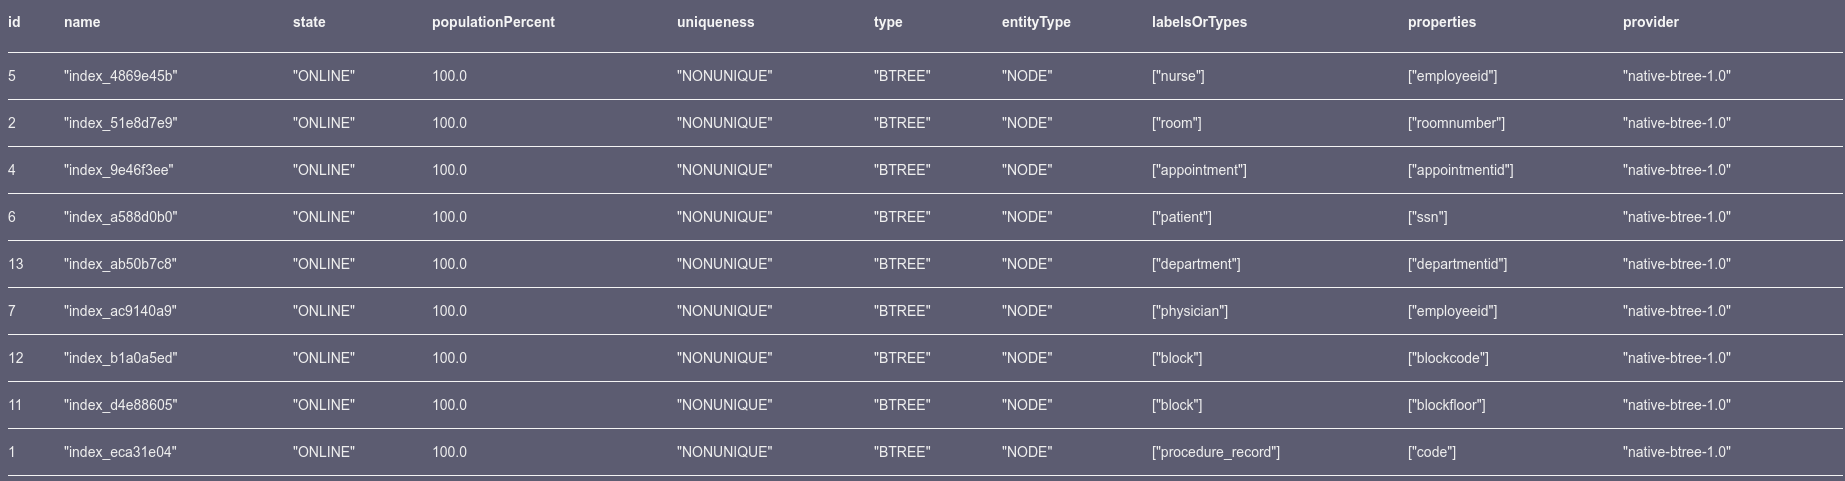
\includegraphics[width=155mm]{img/created_indices.png}
        \caption{Indexes created on test database ``hospital''}
        \label{fig:created_indices}
    \end{figure}

    In figure \ref{fig:created_indices}, we can see the indexes created on the test database. It is essential to note the successful translation of uniqueness constraints and attributes to build B-Tree indexes on the fields as required. Index names are auto-generated.

    \begin{figure}[htb!]
        \centering
        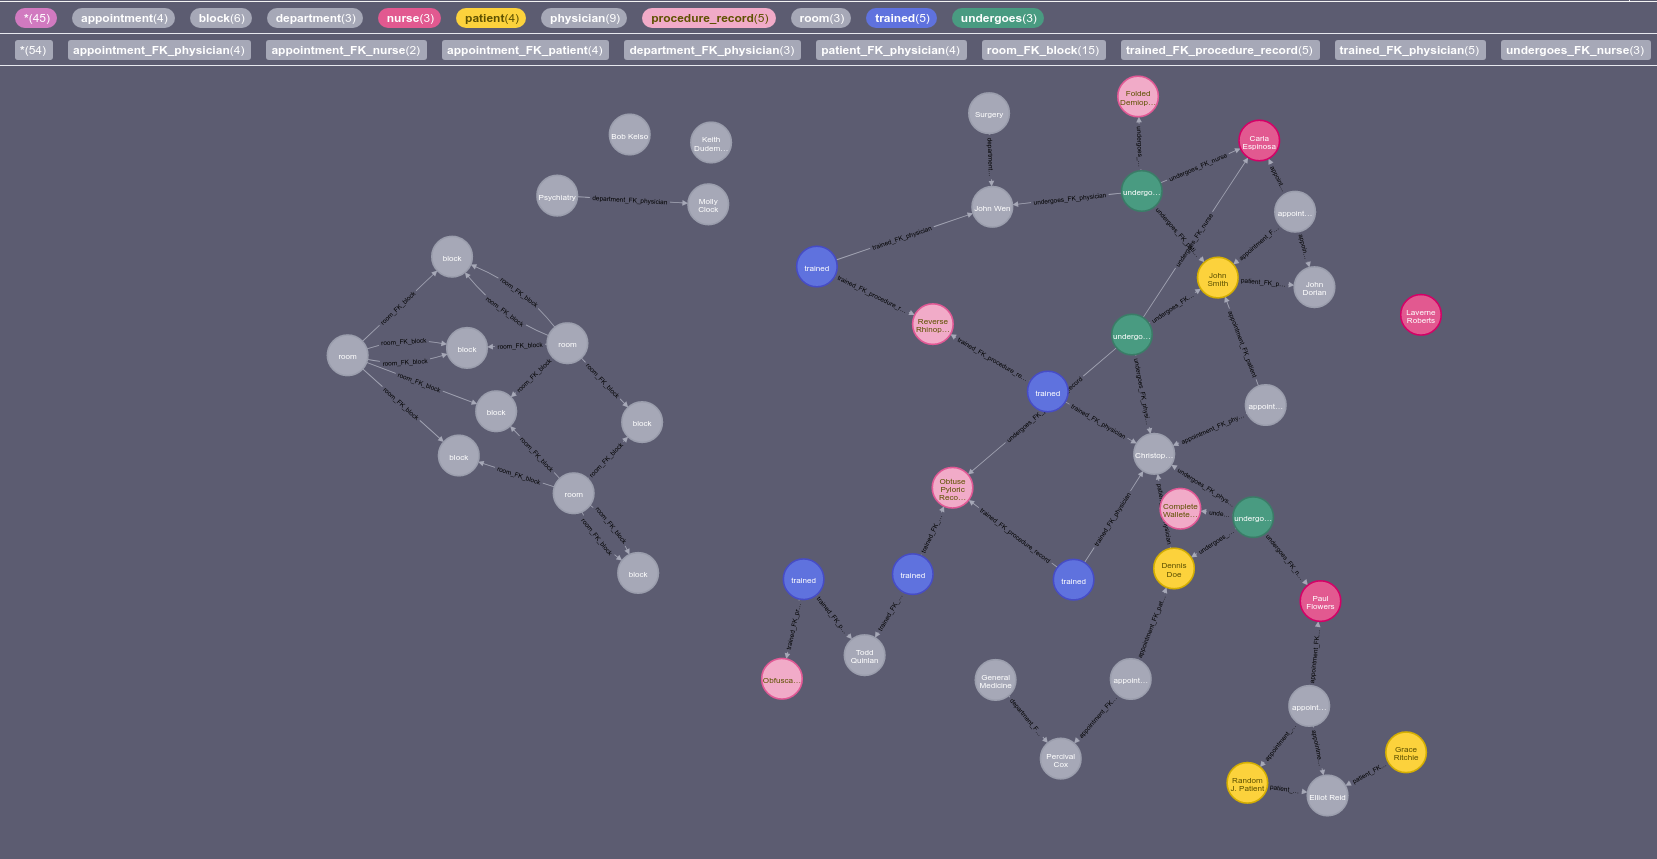
\includegraphics[width=155mm]{img/created_nodes.png}
        \caption{Nodes and relationships created on test database ``hospital''}
        \label{fig:nodes_rels}
    \end{figure}

    In figure \ref{fig:nodes_rels}, we show the successful creation of a graph database with all tables and relations being translated to Neo4j nodes and relations. The entity types are represented by different colored nodes (legend can be found in the top bar of the image), and the labeling of the nodes corresponds to the value in the attribute ``name''. Relationships are represented by a single line joining two nodes with the relationship name written on it. 

    Hovering over an entity will display the additional attributes (apart from ``name'') of the entity. Similarly, we can see additional attributes of relations by hovering over them. 

    For a closer look at the structure of the nodes, we look to figure \ref{fig:node_subset}.

    \begin{figure}[htb!]
        \centering
        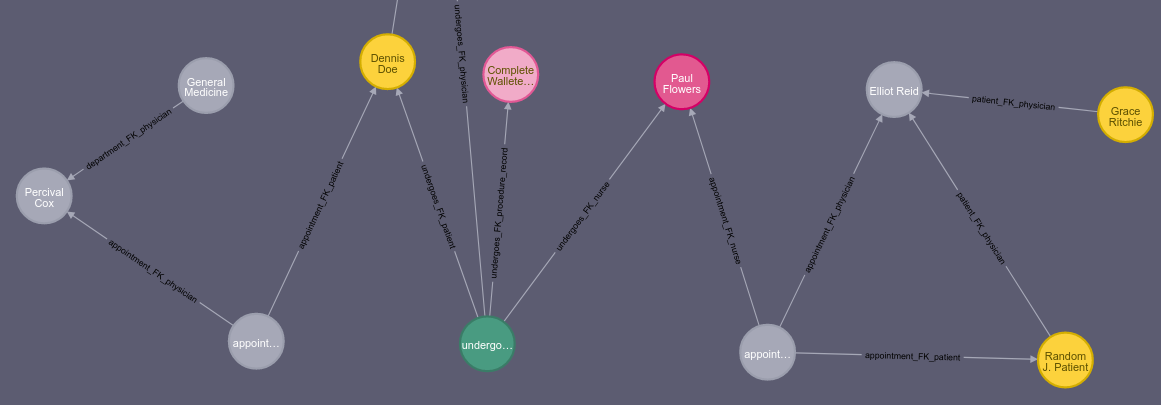
\includegraphics[width=155mm]{img/node_subset.png}
        \caption{View of nodes and relationships created on test database ``hospital''}
        \label{fig:node_subset}
    \end{figure}

    Here we get a better view of the structure of nodes and relationships. As mentioned earlier, nodes are identified by their ``name'' attribute value, and colors represent the entity types. 

    Relationships between have been named according to the convention 
    \begin{lstlisting}
    <from_relation>_FK_<to_relation>    
    \end{lstlisting} 
    to describe the foreign key linking the two tables in the MySQL schema form. ``Relationship Nodes'' have been naively created to represent concepts involving multiple foreign keys such as the ``appointment'' nodes, created to link physician, patient and nurse nodes. Ideally, these relationships should be modeled as links between the nodes, rather than nodes themselves. However, due to challenges faced in the automatic identification of entities vs. relationships, we currently model them, as shown above.

    The output of MongoDB is not shown here since it just creates nodes and indexes. Since no relationship extraction is performed, it is a subset of the output of MySQL migration.

    \newpage

    \section{\sectionfontstyle Conclusion and Future Works}
    In conclusion, it is found that it is feasible to undertake such transformation tasks between SQL/NoSQL databases and that it is also quite beneficial when considering improved data visualization and presentation. The implementation of Sql2Neo discussed is additionally easily extensible to include various other source databases as a result of its system architecture and the use of an intermediate SQL-like data storage strategy.

    Future works include, as mentioned, the extension of this project to bring more source databases within the transformation fold and improve the quality of relationships derived from the data through more inference driven approaches (rather than the naive approach undertaken here). Furthermore, the implementation of a query translator from SQL to CQL will bridge the gap between the two technologies. It will also allow for a more analytical approach to the SQL database and a graphical approach to the Neo4j database. Currently, all indices are single attribute indices and are created only on the primary key (or first unique value for NoSQL). An improvement would be to support composite attribute index conversion. These indices are present in SQL databases and can provide performance improvements in Neo4j as well.

    \newpage

    \bibliographystyle{ieeetr}
    \bibliography{references}
\end{document}